% Graphic for TeX using PGF
% Title: C:\Users\loco\Desktop\studium\10Sem\KlinischeForschung\Modelle\CustomClasses.dia
% Creator: Dia v0.97.2
% CreationDate: Sat Jan 04 13:14:19 2014
% For: loco
% \usepackage{tikz}
% The following commands are not supported in PSTricks at present
% We define them conditionally, so when they are implemented,
% this pgf file will use them.
\ifx\du\undefined
  \newlength{\du}
\fi
\setlength{\du}{22\unitlength}
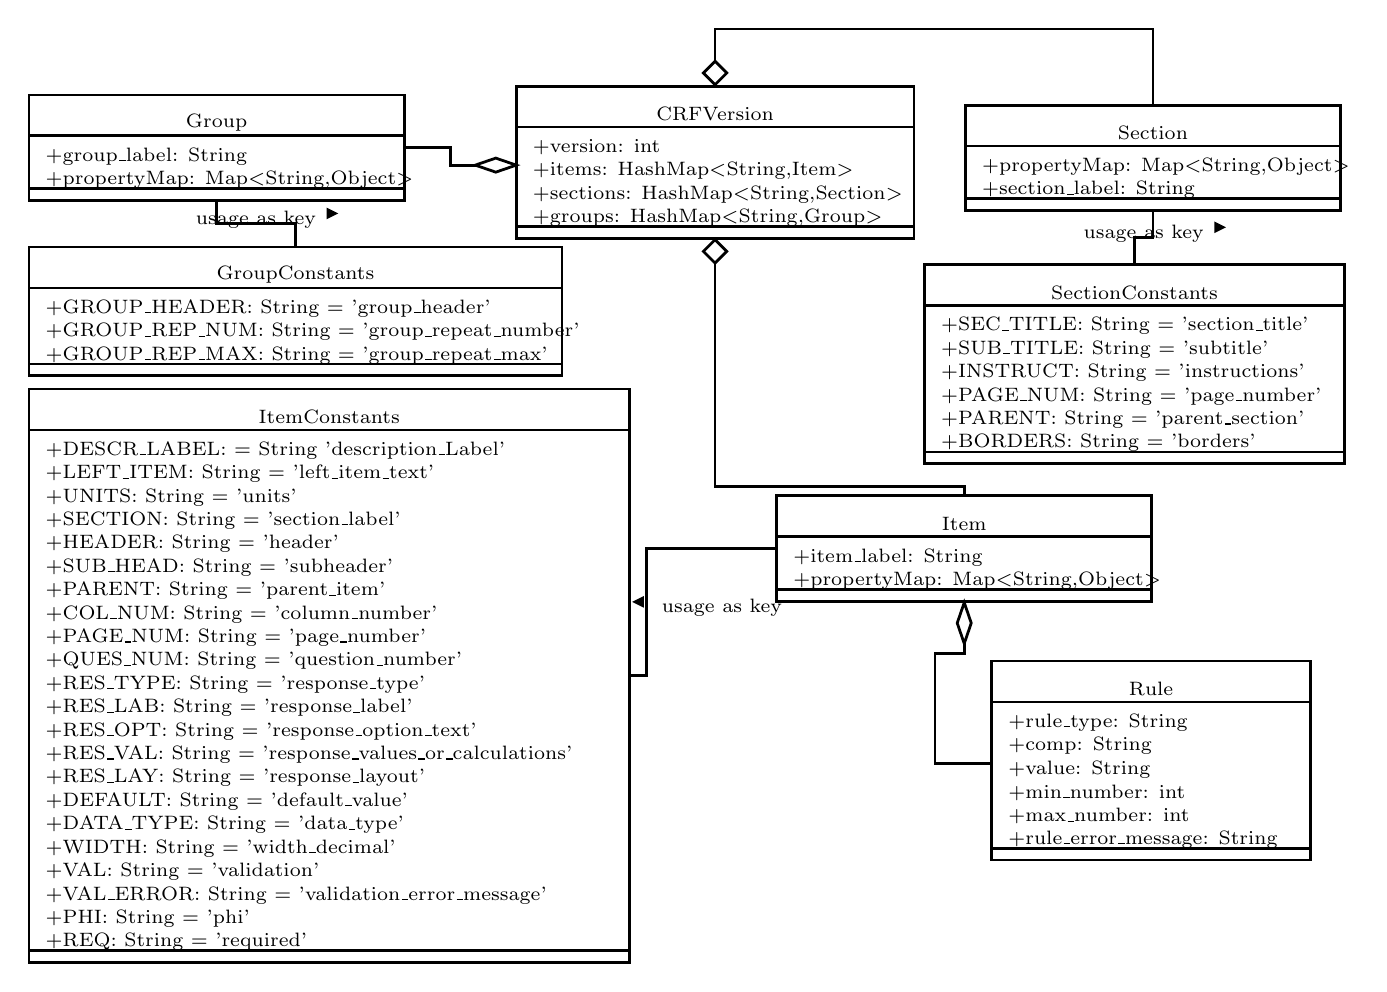
\begin{tikzpicture}
\tikzstyle{every node}=[font=\scriptsize]
\tikzstyle{lw} = [line width=1pt]
\pgftransformxscale{0.480609}
\pgftransformyscale{-0.480609}
\definecolor{dialinecolor}{rgb}{0.000000, 0.000000, 0.000000}
\pgfsetstrokecolor{dialinecolor}
\definecolor{dialinecolor}{rgb}{1.000000, 1.000000, 1.000000}
\pgfsetfillcolor{dialinecolor}
\pgfsetlinewidth{0.100000\du}
\pgfsetdash{}{0pt}
\definecolor{dialinecolor}{rgb}{1.000000, 1.000000, 1.000000}
\pgfsetfillcolor{dialinecolor}
\fill (27.300000\du,14.650000\du)--(27.300000\du,16.050000\du)--(40.120000\du,16.050000\du)--(40.120000\du,14.650000\du)--cycle;
\definecolor{dialinecolor}{rgb}{0.000000, 0.000000, 0.000000}
\pgfsetstrokecolor{dialinecolor}
\draw[lw] (27.300000\du,14.650000\du)--(27.300000\du,16.050000\du)--(40.120000\du,16.050000\du)--(40.120000\du,14.650000\du)--cycle;
% setfont left to latex
\definecolor{dialinecolor}{rgb}{0.000000, 0.000000, 0.000000}
\pgfsetstrokecolor{dialinecolor}
\node at (33.710000\du,15.600000\du){Item};
\definecolor{dialinecolor}{rgb}{1.000000, 1.000000, 1.000000}
\pgfsetfillcolor{dialinecolor}
\fill (27.300000\du,16.050000\du)--(27.300000\du,17.850000\du)--(40.120000\du,17.850000\du)--(40.120000\du,16.050000\du)--cycle;
\definecolor{dialinecolor}{rgb}{0.000000, 0.000000, 0.000000}
\pgfsetstrokecolor{dialinecolor}
\draw[lw] (27.300000\du,16.050000\du)--(27.300000\du,17.850000\du)--(40.120000\du,17.850000\du)--(40.120000\du,16.050000\du)--cycle;
% setfont left to latex
\definecolor{dialinecolor}{rgb}{0.000000, 0.000000, 0.000000}
\pgfsetstrokecolor{dialinecolor}
\node[anchor=west] at (27.450000\du,16.750000\du){+item\_label: String};
% setfont left to latex
\definecolor{dialinecolor}{rgb}{0.000000, 0.000000, 0.000000}
\pgfsetstrokecolor{dialinecolor}
\node[anchor=west] at (27.450000\du,17.550000\du){+propertyMap: Map$<$String,Object$>$};
\definecolor{dialinecolor}{rgb}{1.000000, 1.000000, 1.000000}
\pgfsetfillcolor{dialinecolor}
\fill (27.300000\du,17.850000\du)--(27.300000\du,18.250000\du)--(40.120000\du,18.250000\du)--(40.120000\du,17.850000\du)--cycle;
\definecolor{dialinecolor}{rgb}{0.000000, 0.000000, 0.000000}
\pgfsetstrokecolor{dialinecolor}
\draw[lw] (27.300000\du,17.850000\du)--(27.300000\du,18.250000\du)--(40.120000\du,18.250000\du)--(40.120000\du,17.850000\du)--cycle;
\pgfsetlinewidth{0.100000\du}
\pgfsetdash{}{0pt}
\definecolor{dialinecolor}{rgb}{1.000000, 1.000000, 1.000000}
\pgfsetfillcolor{dialinecolor}
\fill (34.650000\du,20.300000\du)--(34.650000\du,21.700000\du)--(45.545000\du,21.700000\du)--(45.545000\du,20.300000\du)--cycle;
\definecolor{dialinecolor}{rgb}{0.000000, 0.000000, 0.000000}
\pgfsetstrokecolor{dialinecolor}
\draw[lw] (34.650000\du,20.300000\du)--(34.650000\du,21.700000\du)--(45.545000\du,21.700000\du)--(45.545000\du,20.300000\du)--cycle;
% setfont left to latex
\definecolor{dialinecolor}{rgb}{0.000000, 0.000000, 0.000000}
\pgfsetstrokecolor{dialinecolor}
\node at (40.097500\du,21.250000\du){Rule};
\definecolor{dialinecolor}{rgb}{1.000000, 1.000000, 1.000000}
\pgfsetfillcolor{dialinecolor}
\fill (34.650000\du,21.700000\du)--(34.650000\du,26.700000\du)--(45.545000\du,26.700000\du)--(45.545000\du,21.700000\du)--cycle;
\definecolor{dialinecolor}{rgb}{0.000000, 0.000000, 0.000000}
\pgfsetstrokecolor{dialinecolor}
\draw[lw] (34.650000\du,21.700000\du)--(34.650000\du,26.700000\du)--(45.545000\du,26.700000\du)--(45.545000\du,21.700000\du)--cycle;
% setfont left to latex
\definecolor{dialinecolor}{rgb}{0.000000, 0.000000, 0.000000}
\pgfsetstrokecolor{dialinecolor}
\node[anchor=west] at (34.800000\du,22.400000\du){+rule\_type: String};
% setfont left to latex
\definecolor{dialinecolor}{rgb}{0.000000, 0.000000, 0.000000}
\pgfsetstrokecolor{dialinecolor}
\node[anchor=west] at (34.800000\du,23.200000\du){+comp: String};
% setfont left to latex
\definecolor{dialinecolor}{rgb}{0.000000, 0.000000, 0.000000}
\pgfsetstrokecolor{dialinecolor}
\node[anchor=west] at (34.800000\du,24.000000\du){+value: String};
% setfont left to latex
\definecolor{dialinecolor}{rgb}{0.000000, 0.000000, 0.000000}
\pgfsetstrokecolor{dialinecolor}
\node[anchor=west] at (34.800000\du,24.800000\du){+min\_number: int};
% setfont left to latex
\definecolor{dialinecolor}{rgb}{0.000000, 0.000000, 0.000000}
\pgfsetstrokecolor{dialinecolor}
\node[anchor=west] at (34.800000\du,25.600000\du){+max\_number: int};
% setfont left to latex
\definecolor{dialinecolor}{rgb}{0.000000, 0.000000, 0.000000}
\pgfsetstrokecolor{dialinecolor}
\node[anchor=west] at (34.800000\du,26.400000\du){+rule\_error\_message: String};
\definecolor{dialinecolor}{rgb}{1.000000, 1.000000, 1.000000}
\pgfsetfillcolor{dialinecolor}
\fill (34.650000\du,26.700000\du)--(34.650000\du,27.100000\du)--(45.545000\du,27.100000\du)--(45.545000\du,26.700000\du)--cycle;
\definecolor{dialinecolor}{rgb}{0.000000, 0.000000, 0.000000}
\pgfsetstrokecolor{dialinecolor}
\draw[lw] (34.650000\du,26.700000\du)--(34.650000\du,27.100000\du)--(45.545000\du,27.100000\du)--(45.545000\du,26.700000\du)--cycle;
\pgfsetlinewidth{0.100000\du}
\pgfsetdash{}{0pt}
\definecolor{dialinecolor}{rgb}{1.000000, 1.000000, 1.000000}
\pgfsetfillcolor{dialinecolor}
\fill (1.750000\du,11.000000\du)--(1.750000\du,12.400000\du)--(22.270000\du,12.400000\du)--(22.270000\du,11.000000\du)--cycle;
\definecolor{dialinecolor}{rgb}{0.000000, 0.000000, 0.000000}
\pgfsetstrokecolor{dialinecolor}
\draw[lw] (1.750000\du,11.000000\du)--(1.750000\du,12.400000\du)--(22.270000\du,12.400000\du)--(22.270000\du,11.000000\du)--cycle;
% setfont left to latex
\definecolor{dialinecolor}{rgb}{0.000000, 0.000000, 0.000000}
\pgfsetstrokecolor{dialinecolor}
\node at (12.010000\du,11.950000\du){ItemConstants};
\definecolor{dialinecolor}{rgb}{1.000000, 1.000000, 1.000000}
\pgfsetfillcolor{dialinecolor}
\fill (1.750000\du,12.400000\du)--(1.750000\du,30.200000\du)--(22.270000\du,30.200000\du)--(22.270000\du,12.400000\du)--cycle;
\definecolor{dialinecolor}{rgb}{0.000000, 0.000000, 0.000000}
\pgfsetstrokecolor{dialinecolor}
\draw[lw] (1.750000\du,12.400000\du)--(1.750000\du,30.200000\du)--(22.270000\du,30.200000\du)--(22.270000\du,12.400000\du)--cycle;
% setfont left to latex
\definecolor{dialinecolor}{rgb}{0.000000, 0.000000, 0.000000}
\pgfsetstrokecolor{dialinecolor}
\node[anchor=west] at (1.900000\du,13.100000\du){+DESCR\_LABEL: = String  'description\_Label'};
% setfont left to latex
\definecolor{dialinecolor}{rgb}{0.000000, 0.000000, 0.000000}
\pgfsetstrokecolor{dialinecolor}
\node[anchor=west] at (1.900000\du,13.900000\du){+LEFT\_ITEM: String = 'left\_item\_text'};
% setfont left to latex
\definecolor{dialinecolor}{rgb}{0.000000, 0.000000, 0.000000}
\pgfsetstrokecolor{dialinecolor}
\node[anchor=west] at (1.900000\du,14.700000\du){+UNITS: String = 'units'};
% setfont left to latex
\definecolor{dialinecolor}{rgb}{0.000000, 0.000000, 0.000000}
\pgfsetstrokecolor{dialinecolor}
\node[anchor=west] at (1.900000\du,15.500000\du){+SECTION: String = 'section\_label'};
% setfont left to latex
\definecolor{dialinecolor}{rgb}{0.000000, 0.000000, 0.000000}
\pgfsetstrokecolor{dialinecolor}
\node[anchor=west] at (1.900000\du,16.300000\du){+HEADER: String = 'header'};
% setfont left to latex
\definecolor{dialinecolor}{rgb}{0.000000, 0.000000, 0.000000}
\pgfsetstrokecolor{dialinecolor}
\node[anchor=west] at (1.900000\du,17.100000\du){+SUB\_HEAD: String = 'subheader'};
% setfont left to latex
\definecolor{dialinecolor}{rgb}{0.000000, 0.000000, 0.000000}
\pgfsetstrokecolor{dialinecolor}
\node[anchor=west] at (1.900000\du,17.900000\du){+PARENT: String = 'parent\_item'};
% setfont left to latex
\definecolor{dialinecolor}{rgb}{0.000000, 0.000000, 0.000000}
\pgfsetstrokecolor{dialinecolor}
\node[anchor=west] at (1.900000\du,18.700000\du){+COL\_NUM: String = 'column\_number'};
% setfont left to latex
\definecolor{dialinecolor}{rgb}{0.000000, 0.000000, 0.000000}
\pgfsetstrokecolor{dialinecolor}
\node[anchor=west] at (1.900000\du,19.500000\du){+PAGE\_NUM: String = 'page\_number'};
% setfont left to latex
\definecolor{dialinecolor}{rgb}{0.000000, 0.000000, 0.000000}
\pgfsetstrokecolor{dialinecolor}
\node[anchor=west] at (1.900000\du,20.300000\du){+QUES\_NUM: String = 'question\_number'};
% setfont left to latex
\definecolor{dialinecolor}{rgb}{0.000000, 0.000000, 0.000000}
\pgfsetstrokecolor{dialinecolor}
\node[anchor=west] at (1.900000\du,21.100000\du){+RES\_TYPE: String = 'response\_type'};
% setfont left to latex
\definecolor{dialinecolor}{rgb}{0.000000, 0.000000, 0.000000}
\pgfsetstrokecolor{dialinecolor}
\node[anchor=west] at (1.900000\du,21.900000\du){+RES\_LAB: String = 'response\_label'};
% setfont left to latex
\definecolor{dialinecolor}{rgb}{0.000000, 0.000000, 0.000000}
\pgfsetstrokecolor{dialinecolor}
\node[anchor=west] at (1.900000\du,22.700000\du){+RES\_OPT: String = 'response\_option\_text'};
% setfont left to latex
\definecolor{dialinecolor}{rgb}{0.000000, 0.000000, 0.000000}
\pgfsetstrokecolor{dialinecolor}
\node[anchor=west] at (1.900000\du,23.500000\du){+RES\_VAL: String = 'response\_values\_or\_calculations'};
% setfont left to latex
\definecolor{dialinecolor}{rgb}{0.000000, 0.000000, 0.000000}
\pgfsetstrokecolor{dialinecolor}
\node[anchor=west] at (1.900000\du,24.300000\du){+RES\_LAY: String = 'response\_layout'};
% setfont left to latex
\definecolor{dialinecolor}{rgb}{0.000000, 0.000000, 0.000000}
\pgfsetstrokecolor{dialinecolor}
\node[anchor=west] at (1.900000\du,25.100000\du){+DEFAULT: String = 'default\_value'};
% setfont left to latex
\definecolor{dialinecolor}{rgb}{0.000000, 0.000000, 0.000000}
\pgfsetstrokecolor{dialinecolor}
\node[anchor=west] at (1.900000\du,25.900000\du){+DATA\_TYPE: String = 'data\_type'};
% setfont left to latex
\definecolor{dialinecolor}{rgb}{0.000000, 0.000000, 0.000000}
\pgfsetstrokecolor{dialinecolor}
\node[anchor=west] at (1.900000\du,26.700000\du){+WIDTH: String = 'width\_decimal'};
% setfont left to latex
\definecolor{dialinecolor}{rgb}{0.000000, 0.000000, 0.000000}
\pgfsetstrokecolor{dialinecolor}
\node[anchor=west] at (1.900000\du,27.500000\du){+VAL: String = 'validation'};
% setfont left to latex
\definecolor{dialinecolor}{rgb}{0.000000, 0.000000, 0.000000}
\pgfsetstrokecolor{dialinecolor}
\node[anchor=west] at (1.900000\du,28.300000\du){+VAL\_ERROR: String = 'validation\_error\_message'};
% setfont left to latex
\definecolor{dialinecolor}{rgb}{0.000000, 0.000000, 0.000000}
\pgfsetstrokecolor{dialinecolor}
\node[anchor=west] at (1.900000\du,29.100000\du){+PHI: String = 'phi'};
% setfont left to latex
\definecolor{dialinecolor}{rgb}{0.000000, 0.000000, 0.000000}
\pgfsetstrokecolor{dialinecolor}
\node[anchor=west] at (1.900000\du,29.900000\du){+REQ: String = 'required'};
\definecolor{dialinecolor}{rgb}{1.000000, 1.000000, 1.000000}
\pgfsetfillcolor{dialinecolor}
\fill (1.750000\du,30.200000\du)--(1.750000\du,30.600000\du)--(22.270000\du,30.600000\du)--(22.270000\du,30.200000\du)--cycle;
\definecolor{dialinecolor}{rgb}{0.000000, 0.000000, 0.000000}
\pgfsetstrokecolor{dialinecolor}
\draw[lw] (1.750000\du,30.200000\du)--(1.750000\du,30.600000\du)--(22.270000\du,30.600000\du)--(22.270000\du,30.200000\du)--cycle;
\pgfsetlinewidth{0.100000\du}
\pgfsetdash{}{0pt}
\pgfsetmiterjoin
\pgfsetbuttcap
{
\definecolor{dialinecolor}{rgb}{0.000000, 0.000000, 0.000000}
\pgfsetfillcolor{dialinecolor}
% was here!!!
\definecolor{dialinecolor}{rgb}{0.000000, 0.000000, 0.000000}
\pgfsetstrokecolor{dialinecolor}
\draw[lw] (33.710000\du,18.300452\du)--(33.710000\du,20.050452\du)--(32.710000\du,20.050452\du)--(32.710000\du,23.800000\du)--(34.650000\du,23.800000\du);
}
\definecolor{dialinecolor}{rgb}{0.000000, 0.000000, 0.000000}
\pgfsetstrokecolor{dialinecolor}
\draw[lw] (33.710000\du,19.559030\du)--(33.710000\du,20.050452\du)--(32.710000\du,20.050452\du)--(32.710000\du,23.800000\du)--(34.650000\du,23.800000\du);
\pgfsetdash{}{0pt}
\pgfsetmiterjoin
\pgfsetbuttcap
\definecolor{dialinecolor}{rgb}{1.000000, 1.000000, 1.000000}
\pgfsetfillcolor{dialinecolor}
\fill (33.710000\du,18.300452\du)--(33.950000\du,19.000452\du)--(33.710000\du,19.700452\du)--(33.470000\du,19.000452\du)--cycle;
\pgfsetlinewidth{0.100000\du}
\pgfsetdash{}{0pt}
\pgfsetmiterjoin
\pgfsetbuttcap
\definecolor{dialinecolor}{rgb}{0.000000, 0.000000, 0.000000}
\pgfsetstrokecolor{dialinecolor}
\draw[lw] (33.710000\du,18.300452\du)--(33.950000\du,19.000452\du)--(33.710000\du,19.700452\du)--(33.470000\du,19.000452\du)--cycle;
% setfont left to latex
\definecolor{dialinecolor}{rgb}{0.000000, 0.000000, 0.000000}
\pgfsetstrokecolor{dialinecolor}
\node at (33.210000\du,19.900452\du){};
\definecolor{dialinecolor}{rgb}{0.000000, 0.000000, 0.000000}
\pgfsetstrokecolor{dialinecolor}
\node[anchor=west] at (34.260000\du,18.900452\du){};
\definecolor{dialinecolor}{rgb}{0.000000, 0.000000, 0.000000}
\pgfsetstrokecolor{dialinecolor}
\node[anchor=east] at (34.450000\du,23.650000\du){};
\pgfsetlinewidth{0.100000\du}
\pgfsetdash{}{0pt}
\pgfsetmiterjoin
\pgfsetbuttcap
{
\definecolor{dialinecolor}{rgb}{0.000000, 0.000000, 0.000000}
\pgfsetfillcolor{dialinecolor}
% was here!!!
\definecolor{dialinecolor}{rgb}{0.000000, 0.000000, 0.000000}
\pgfsetstrokecolor{dialinecolor}
\draw[lw] (22.320281\du,20.800000\du)--(22.860000\du,20.800000\du)--(22.860000\du,16.450000\du)--(27.250594\du,16.450000\du);
}
% setfont left to latex
\definecolor{dialinecolor}{rgb}{0.000000, 0.000000, 0.000000}
\pgfsetstrokecolor{dialinecolor}
\node[anchor=west] at (22.960000\du,18.475000\du){usage as key};
\definecolor{dialinecolor}{rgb}{0.000000, 0.000000, 0.000000}
\pgfsetfillcolor{dialinecolor}
\fill (22.760000\du,18.475000\du)--(22.760000\du,18.075000\du)--(22.360000\du,18.275000\du)--cycle;
\definecolor{dialinecolor}{rgb}{0.000000, 0.000000, 0.000000}
\pgfsetstrokecolor{dialinecolor}
\node[anchor=west] at (22.520281\du,20.650000\du){};
\definecolor{dialinecolor}{rgb}{0.000000, 0.000000, 0.000000}
\pgfsetstrokecolor{dialinecolor}
\node[anchor=east] at (27.050594\du,16.300000\du){};
\pgfsetlinewidth{0.100000\du}
\pgfsetdash{}{0pt}
\definecolor{dialinecolor}{rgb}{1.000000, 1.000000, 1.000000}
\pgfsetfillcolor{dialinecolor}
\fill (33.750000\du,1.300010\du)--(33.750000\du,2.700010\du)--(46.570000\du,2.700010\du)--(46.570000\du,1.300010\du)--cycle;
\definecolor{dialinecolor}{rgb}{0.000000, 0.000000, 0.000000}
\pgfsetstrokecolor{dialinecolor}
\draw[lw] (33.750000\du,1.300010\du)--(33.750000\du,2.700010\du)--(46.570000\du,2.700010\du)--(46.570000\du,1.300010\du)--cycle;
% setfont left to latex
\definecolor{dialinecolor}{rgb}{0.000000, 0.000000, 0.000000}
\pgfsetstrokecolor{dialinecolor}
\node at (40.160000\du,2.250010\du){Section};
\definecolor{dialinecolor}{rgb}{1.000000, 1.000000, 1.000000}
\pgfsetfillcolor{dialinecolor}
\fill (33.750000\du,2.700010\du)--(33.750000\du,4.500010\du)--(46.570000\du,4.500010\du)--(46.570000\du,2.700010\du)--cycle;
\definecolor{dialinecolor}{rgb}{0.000000, 0.000000, 0.000000}
\pgfsetstrokecolor{dialinecolor}
\draw[lw] (33.750000\du,2.700010\du)--(33.750000\du,4.500010\du)--(46.570000\du,4.500010\du)--(46.570000\du,2.700010\du)--cycle;
% setfont left to latex
\definecolor{dialinecolor}{rgb}{0.000000, 0.000000, 0.000000}
\pgfsetstrokecolor{dialinecolor}
\node[anchor=west] at (33.900000\du,3.400010\du){+propertyMap: Map$<$String,Object$>$};
% setfont left to latex
\definecolor{dialinecolor}{rgb}{0.000000, 0.000000, 0.000000}
\pgfsetstrokecolor{dialinecolor}
\node[anchor=west] at (33.900000\du,4.200010\du){+section\_label: String};
\definecolor{dialinecolor}{rgb}{1.000000, 1.000000, 1.000000}
\pgfsetfillcolor{dialinecolor}
\fill (33.750000\du,4.500010\du)--(33.750000\du,4.900010\du)--(46.570000\du,4.900010\du)--(46.570000\du,4.500010\du)--cycle;
\definecolor{dialinecolor}{rgb}{0.000000, 0.000000, 0.000000}
\pgfsetstrokecolor{dialinecolor}
\draw[lw] (33.750000\du,4.500010\du)--(33.750000\du,4.900010\du)--(46.570000\du,4.900010\du)--(46.570000\du,4.500010\du)--cycle;
\pgfsetlinewidth{0.100000\du}
\pgfsetdash{}{0pt}
\definecolor{dialinecolor}{rgb}{1.000000, 1.000000, 1.000000}
\pgfsetfillcolor{dialinecolor}
\fill (32.350000\du,6.750010\du)--(32.350000\du,8.150010\du)--(46.710000\du,8.150010\du)--(46.710000\du,6.750010\du)--cycle;
\definecolor{dialinecolor}{rgb}{0.000000, 0.000000, 0.000000}
\pgfsetstrokecolor{dialinecolor}
\draw[lw] (32.350000\du,6.750010\du)--(32.350000\du,8.150010\du)--(46.710000\du,8.150010\du)--(46.710000\du,6.750010\du)--cycle;
% setfont left to latex
\definecolor{dialinecolor}{rgb}{0.000000, 0.000000, 0.000000}
\pgfsetstrokecolor{dialinecolor}
\node at (39.530000\du,7.700010\du){SectionConstants};
\definecolor{dialinecolor}{rgb}{1.000000, 1.000000, 1.000000}
\pgfsetfillcolor{dialinecolor}
\fill (32.350000\du,8.150010\du)--(32.350000\du,13.150010\du)--(46.710000\du,13.150010\du)--(46.710000\du,8.150010\du)--cycle;
\definecolor{dialinecolor}{rgb}{0.000000, 0.000000, 0.000000}
\pgfsetstrokecolor{dialinecolor}
\draw[lw] (32.350000\du,8.150010\du)--(32.350000\du,13.150010\du)--(46.710000\du,13.150010\du)--(46.710000\du,8.150010\du)--cycle;
% setfont left to latex
\definecolor{dialinecolor}{rgb}{0.000000, 0.000000, 0.000000}
\pgfsetstrokecolor{dialinecolor}
\node[anchor=west] at (32.500000\du,8.850010\du){+SEC\_TITLE: String = 'section\_title'};
% setfont left to latex
\definecolor{dialinecolor}{rgb}{0.000000, 0.000000, 0.000000}
\pgfsetstrokecolor{dialinecolor}
\node[anchor=west] at (32.500000\du,9.650010\du){+SUB\_TITLE: String = 'subtitle'};
% setfont left to latex
\definecolor{dialinecolor}{rgb}{0.000000, 0.000000, 0.000000}
\pgfsetstrokecolor{dialinecolor}
\node[anchor=west] at (32.500000\du,10.450010\du){+INSTRUCT: String = 'instructions'};
% setfont left to latex
\definecolor{dialinecolor}{rgb}{0.000000, 0.000000, 0.000000}
\pgfsetstrokecolor{dialinecolor}
\node[anchor=west] at (32.500000\du,11.250010\du){+PAGE\_NUM: String = 'page\_number'};
% setfont left to latex
\definecolor{dialinecolor}{rgb}{0.000000, 0.000000, 0.000000}
\pgfsetstrokecolor{dialinecolor}
\node[anchor=west] at (32.500000\du,12.050010\du){+PARENT: String = 'parent\_section'};
% setfont left to latex
\definecolor{dialinecolor}{rgb}{0.000000, 0.000000, 0.000000}
\pgfsetstrokecolor{dialinecolor}
\node[anchor=west] at (32.500000\du,12.850010\du){+BORDERS: String = 'borders'};
\definecolor{dialinecolor}{rgb}{1.000000, 1.000000, 1.000000}
\pgfsetfillcolor{dialinecolor}
\fill (32.350000\du,13.150010\du)--(32.350000\du,13.550010\du)--(46.710000\du,13.550010\du)--(46.710000\du,13.150010\du)--cycle;
\definecolor{dialinecolor}{rgb}{0.000000, 0.000000, 0.000000}
\pgfsetstrokecolor{dialinecolor}
\draw[lw] (32.350000\du,13.150010\du)--(32.350000\du,13.550010\du)--(46.710000\du,13.550010\du)--(46.710000\du,13.150010\du)--cycle;
\pgfsetlinewidth{0.100000\du}
\pgfsetdash{}{0pt}
\definecolor{dialinecolor}{rgb}{1.000000, 1.000000, 1.000000}
\pgfsetfillcolor{dialinecolor}
\fill (18.400000\du,0.650010\du)--(18.400000\du,2.050010\du)--(31.990000\du,2.050010\du)--(31.990000\du,0.650010\du)--cycle;
\definecolor{dialinecolor}{rgb}{0.000000, 0.000000, 0.000000}
\pgfsetstrokecolor{dialinecolor}
\draw[lw] (18.400000\du,0.650010\du)--(18.400000\du,2.050010\du)--(31.990000\du,2.050010\du)--(31.990000\du,0.650010\du)--cycle;
% setfont left to latex
\definecolor{dialinecolor}{rgb}{0.000000, 0.000000, 0.000000}
\pgfsetstrokecolor{dialinecolor}
\node at (25.195000\du,1.600010\du){CRFVersion};
\definecolor{dialinecolor}{rgb}{1.000000, 1.000000, 1.000000}
\pgfsetfillcolor{dialinecolor}
\fill (18.400000\du,2.050010\du)--(18.400000\du,5.450010\du)--(31.990000\du,5.450010\du)--(31.990000\du,2.050010\du)--cycle;
\definecolor{dialinecolor}{rgb}{0.000000, 0.000000, 0.000000}
\pgfsetstrokecolor{dialinecolor}
\draw[lw] (18.400000\du,2.050010\du)--(18.400000\du,5.450010\du)--(31.990000\du,5.450010\du)--(31.990000\du,2.050010\du)--cycle;
% setfont left to latex
\definecolor{dialinecolor}{rgb}{0.000000, 0.000000, 0.000000}
\pgfsetstrokecolor{dialinecolor}
\node[anchor=west] at (18.550000\du,2.750010\du){+version: int};
% setfont left to latex
\definecolor{dialinecolor}{rgb}{0.000000, 0.000000, 0.000000}
\pgfsetstrokecolor{dialinecolor}
\node[anchor=west] at (18.550000\du,3.550010\du){+items: HashMap$<$String,Item$>$};
% setfont left to latex
\definecolor{dialinecolor}{rgb}{0.000000, 0.000000, 0.000000}
\pgfsetstrokecolor{dialinecolor}
\node[anchor=west] at (18.550000\du,4.350010\du){+sections: HashMap$<$String,Section$>$};
% setfont left to latex
\definecolor{dialinecolor}{rgb}{0.000000, 0.000000, 0.000000}
\pgfsetstrokecolor{dialinecolor}
\node[anchor=west] at (18.550000\du,5.150010\du){+groups: HashMap$<$String,Group$>$};
\definecolor{dialinecolor}{rgb}{1.000000, 1.000000, 1.000000}
\pgfsetfillcolor{dialinecolor}
\fill (18.400000\du,5.450010\du)--(18.400000\du,5.850010\du)--(31.990000\du,5.850010\du)--(31.990000\du,5.450010\du)--cycle;
\definecolor{dialinecolor}{rgb}{0.000000, 0.000000, 0.000000}
\pgfsetstrokecolor{dialinecolor}
\draw[lw] (18.400000\du,5.450010\du)--(18.400000\du,5.850010\du)--(31.990000\du,5.850010\du)--(31.990000\du,5.450010\du)--cycle;
\pgfsetlinewidth{0.100000\du}
\pgfsetdash{}{0pt}
\pgfsetbuttcap
{
\definecolor{dialinecolor}{rgb}{0.000000, 0.000000, 0.000000}
\pgfsetfillcolor{dialinecolor}
% was here!!!
\definecolor{dialinecolor}{rgb}{0.000000, 0.000000, 0.000000}
\pgfsetstrokecolor{dialinecolor}
\draw[lw] (40.160000\du,1.249558\du)--(40.160000\du,-1.300313\du)--(25.195000\du,-1.300313\du)--(25.195000\du,0.599687\du);
}
\definecolor{dialinecolor}{rgb}{0.000000, 0.000000, 0.000000}
\pgfsetstrokecolor{dialinecolor}
\draw[lw] (40.160000\du,1.249558\du)--(40.160000\du,-1.300313\du)--(25.195000\du,-1.300313\du)--(25.195000\du,-0.058892\du);
\pgfsetdash{}{0pt}
\pgfsetmiterjoin
\pgfsetbuttcap
\definecolor{dialinecolor}{rgb}{1.000000, 1.000000, 1.000000}
\pgfsetfillcolor{dialinecolor}
\fill (25.195000\du,0.599687\du)--(24.795000\du,0.199687\du)--(25.195000\du,-0.200313\du)--(25.595000\du,0.199687\du)--cycle;
\pgfsetlinewidth{0.100000\du}
\pgfsetdash{}{0pt}
\pgfsetmiterjoin
\pgfsetbuttcap
\definecolor{dialinecolor}{rgb}{0.000000, 0.000000, 0.000000}
\pgfsetstrokecolor{dialinecolor}
\draw[lw] (25.195000\du,0.599687\du)--(24.795000\du,0.199687\du)--(25.195000\du,-0.200313\du)--(25.595000\du,0.199687\du)--cycle;
% setfont left to latex
\definecolor{dialinecolor}{rgb}{0.000000, 0.000000, 0.000000}
\pgfsetstrokecolor{dialinecolor}
\node at (39.900000\du,3.850010\du){};
\pgfsetlinewidth{0.100000\du}
\pgfsetdash{}{0pt}
\pgfsetbuttcap
{
\definecolor{dialinecolor}{rgb}{0.000000, 0.000000, 0.000000}
\pgfsetfillcolor{dialinecolor}
% was here!!!
\definecolor{dialinecolor}{rgb}{0.000000, 0.000000, 0.000000}
\pgfsetstrokecolor{dialinecolor}
\draw[lw] (33.710000\du,14.600531\du)--(33.710000\du,14.337500\du)--(25.195000\du,14.337500\du)--(25.195000\du,5.898718\du);
}
\definecolor{dialinecolor}{rgb}{0.000000, 0.000000, 0.000000}
\pgfsetstrokecolor{dialinecolor}
\draw[lw] (33.710000\du,14.600531\du)--(33.710000\du,14.337500\du)--(25.195000\du,14.337500\du)--(25.195000\du,6.557297\du);
\pgfsetdash{}{0pt}
\pgfsetmiterjoin
\pgfsetbuttcap
\definecolor{dialinecolor}{rgb}{1.000000, 1.000000, 1.000000}
\pgfsetfillcolor{dialinecolor}
\fill (25.195000\du,5.898718\du)--(25.595000\du,6.298718\du)--(25.195000\du,6.698718\du)--(24.795000\du,6.298718\du)--cycle;
\pgfsetlinewidth{0.100000\du}
\pgfsetdash{}{0pt}
\pgfsetmiterjoin
\pgfsetbuttcap
\definecolor{dialinecolor}{rgb}{0.000000, 0.000000, 0.000000}
\pgfsetstrokecolor{dialinecolor}
\draw[lw] (25.195000\du,5.898718\du)--(25.595000\du,6.298718\du)--(25.195000\du,6.698718\du)--(24.795000\du,6.298718\du)--cycle;
% setfont left to latex
\definecolor{dialinecolor}{rgb}{0.000000, 0.000000, 0.000000}
\pgfsetstrokecolor{dialinecolor}
\node at (27.500000\du,11.387500\du){};
\pgfsetlinewidth{0.100000\du}
\pgfsetdash{}{0pt}
\pgfsetmiterjoin
\pgfsetbuttcap
{
\definecolor{dialinecolor}{rgb}{0.000000, 0.000000, 0.000000}
\pgfsetfillcolor{dialinecolor}
% was here!!!
\definecolor{dialinecolor}{rgb}{0.000000, 0.000000, 0.000000}
\pgfsetstrokecolor{dialinecolor}
\draw[lw] (40.160000\du,4.950462\du)--(40.160000\du,5.825025\du)--(39.530000\du,5.825025\du)--(39.530000\du,6.699589\du);
}
% setfont left to latex
\definecolor{dialinecolor}{rgb}{0.000000, 0.000000, 0.000000}
\pgfsetstrokecolor{dialinecolor}
\node at (39.845000\du,5.675025\du){usage as key};
\definecolor{dialinecolor}{rgb}{0.000000, 0.000000, 0.000000}
\pgfsetfillcolor{dialinecolor}
\fill (42.255000\du,5.675025\du)--(42.255000\du,5.275025\du)--(42.655000\du,5.475025\du)--cycle;
\definecolor{dialinecolor}{rgb}{0.000000, 0.000000, 0.000000}
\pgfsetstrokecolor{dialinecolor}
\node[anchor=west] at (40.360000\du,5.550462\du){};
\definecolor{dialinecolor}{rgb}{0.000000, 0.000000, 0.000000}
\pgfsetstrokecolor{dialinecolor}
\node[anchor=west] at (39.730000\du,6.499589\du){};
\pgfsetlinewidth{0.100000\du}
\pgfsetdash{}{0pt}
\definecolor{dialinecolor}{rgb}{1.000000, 1.000000, 1.000000}
\pgfsetfillcolor{dialinecolor}
\fill (1.750000\du,0.950010\du)--(1.750000\du,2.350010\du)--(14.570000\du,2.350010\du)--(14.570000\du,0.950010\du)--cycle;
\definecolor{dialinecolor}{rgb}{0.000000, 0.000000, 0.000000}
\pgfsetstrokecolor{dialinecolor}
\draw[lw] (1.750000\du,0.950010\du)--(1.750000\du,2.350010\du)--(14.570000\du,2.350010\du)--(14.570000\du,0.950010\du)--cycle;
% setfont left to latex
\definecolor{dialinecolor}{rgb}{0.000000, 0.000000, 0.000000}
\pgfsetstrokecolor{dialinecolor}
\node at (8.160000\du,1.900010\du){Group};
\definecolor{dialinecolor}{rgb}{1.000000, 1.000000, 1.000000}
\pgfsetfillcolor{dialinecolor}
\fill (1.750000\du,2.350010\du)--(1.750000\du,4.150010\du)--(14.570000\du,4.150010\du)--(14.570000\du,2.350010\du)--cycle;
\definecolor{dialinecolor}{rgb}{0.000000, 0.000000, 0.000000}
\pgfsetstrokecolor{dialinecolor}
\draw[lw] (1.750000\du,2.350010\du)--(1.750000\du,4.150010\du)--(14.570000\du,4.150010\du)--(14.570000\du,2.350010\du)--cycle;
% setfont left to latex
\definecolor{dialinecolor}{rgb}{0.000000, 0.000000, 0.000000}
\pgfsetstrokecolor{dialinecolor}
\node[anchor=west] at (1.900000\du,3.050010\du){+group\_label: String};
% setfont left to latex
\definecolor{dialinecolor}{rgb}{0.000000, 0.000000, 0.000000}
\pgfsetstrokecolor{dialinecolor}
\node[anchor=west] at (1.900000\du,3.850010\du){+propertyMap: Map$<$String,Object$>$};
\definecolor{dialinecolor}{rgb}{1.000000, 1.000000, 1.000000}
\pgfsetfillcolor{dialinecolor}
\fill (1.750000\du,4.150010\du)--(1.750000\du,4.550010\du)--(14.570000\du,4.550010\du)--(14.570000\du,4.150010\du)--cycle;
\definecolor{dialinecolor}{rgb}{0.000000, 0.000000, 0.000000}
\pgfsetstrokecolor{dialinecolor}
\draw[lw] (1.750000\du,4.150010\du)--(1.750000\du,4.550010\du)--(14.570000\du,4.550010\du)--(14.570000\du,4.150010\du)--cycle;
\pgfsetlinewidth{0.100000\du}
\pgfsetdash{}{0pt}
\definecolor{dialinecolor}{rgb}{1.000000, 1.000000, 1.000000}
\pgfsetfillcolor{dialinecolor}
\fill (1.750000\du,6.150010\du)--(1.750000\du,7.550010\du)--(19.960000\du,7.550010\du)--(19.960000\du,6.150010\du)--cycle;
\definecolor{dialinecolor}{rgb}{0.000000, 0.000000, 0.000000}
\pgfsetstrokecolor{dialinecolor}
\draw[lw] (1.750000\du,6.150010\du)--(1.750000\du,7.550010\du)--(19.960000\du,7.550010\du)--(19.960000\du,6.150010\du)--cycle;
% setfont left to latex
\definecolor{dialinecolor}{rgb}{0.000000, 0.000000, 0.000000}
\pgfsetstrokecolor{dialinecolor}
\node at (10.855000\du,7.100010\du){GroupConstants};
\definecolor{dialinecolor}{rgb}{1.000000, 1.000000, 1.000000}
\pgfsetfillcolor{dialinecolor}
\fill (1.750000\du,7.550010\du)--(1.750000\du,10.150010\du)--(19.960000\du,10.150010\du)--(19.960000\du,7.550010\du)--cycle;
\definecolor{dialinecolor}{rgb}{0.000000, 0.000000, 0.000000}
\pgfsetstrokecolor{dialinecolor}
\draw[lw] (1.750000\du,7.550010\du)--(1.750000\du,10.150010\du)--(19.960000\du,10.150010\du)--(19.960000\du,7.550010\du)--cycle;
% setfont left to latex
\definecolor{dialinecolor}{rgb}{0.000000, 0.000000, 0.000000}
\pgfsetstrokecolor{dialinecolor}
\node[anchor=west] at (1.900000\du,8.250010\du){+GROUP\_HEADER: String = 'group\_header'};
% setfont left to latex
\definecolor{dialinecolor}{rgb}{0.000000, 0.000000, 0.000000}
\pgfsetstrokecolor{dialinecolor}
\node[anchor=west] at (1.900000\du,9.050010\du){+GROUP\_REP\_NUM: String = 'group\_repeat\_number'};
% setfont left to latex
\definecolor{dialinecolor}{rgb}{0.000000, 0.000000, 0.000000}
\pgfsetstrokecolor{dialinecolor}
\node[anchor=west] at (1.900000\du,9.850010\du){+GROUP\_REP\_MAX: String = 'group\_repeat\_max'};
\definecolor{dialinecolor}{rgb}{1.000000, 1.000000, 1.000000}
\pgfsetfillcolor{dialinecolor}
\fill (1.750000\du,10.150010\du)--(1.750000\du,10.550010\du)--(19.960000\du,10.550010\du)--(19.960000\du,10.150010\du)--cycle;
\definecolor{dialinecolor}{rgb}{0.000000, 0.000000, 0.000000}
\pgfsetstrokecolor{dialinecolor}
\draw[lw] (1.750000\du,10.150010\du)--(1.750000\du,10.550010\du)--(19.960000\du,10.550010\du)--(19.960000\du,10.150010\du)--cycle;
\pgfsetlinewidth{0.100000\du}
\pgfsetdash{}{0pt}
\pgfsetmiterjoin
\pgfsetbuttcap
{
\definecolor{dialinecolor}{rgb}{0.000000, 0.000000, 0.000000}
\pgfsetfillcolor{dialinecolor}
% was here!!!
\definecolor{dialinecolor}{rgb}{0.000000, 0.000000, 0.000000}
\pgfsetstrokecolor{dialinecolor}
\draw[lw] (10.855000\du,6.099735\du)--(10.855000\du,5.350099\du)--(8.160000\du,5.350099\du)--(8.160000\du,4.600462\du);
}
% setfont left to latex
\definecolor{dialinecolor}{rgb}{0.000000, 0.000000, 0.000000}
\pgfsetstrokecolor{dialinecolor}
\node at (9.507500\du,5.200099\du){usage as key};
\definecolor{dialinecolor}{rgb}{0.000000, 0.000000, 0.000000}
\pgfsetfillcolor{dialinecolor}
\fill (11.917500\du,5.200099\du)--(11.917500\du,4.800099\du)--(12.317500\du,5.000099\du)--cycle;
\definecolor{dialinecolor}{rgb}{0.000000, 0.000000, 0.000000}
\pgfsetstrokecolor{dialinecolor}
\node[anchor=west] at (11.055000\du,5.899735\du){};
\definecolor{dialinecolor}{rgb}{0.000000, 0.000000, 0.000000}
\pgfsetstrokecolor{dialinecolor}
\node[anchor=west] at (8.360000\du,5.200462\du){};
\pgfsetlinewidth{0.100000\du}
\pgfsetdash{}{0pt}
\pgfsetmiterjoin
\pgfsetbuttcap
{
\definecolor{dialinecolor}{rgb}{0.000000, 0.000000, 0.000000}
\pgfsetfillcolor{dialinecolor}
% was here!!!
\definecolor{dialinecolor}{rgb}{0.000000, 0.000000, 0.000000}
\pgfsetstrokecolor{dialinecolor}
\draw[lw] (18.400000\du,3.350010\du)--(16.160197\du,3.350010\du)--(16.160197\du,2.750010\du)--(14.620394\du,2.750010\du);
}
\definecolor{dialinecolor}{rgb}{0.000000, 0.000000, 0.000000}
\pgfsetstrokecolor{dialinecolor}
\draw[lw] (17.141421\du,3.350010\du)--(16.160197\du,3.350010\du)--(16.160197\du,2.750010\du)--(14.620394\du,2.750010\du);
\pgfsetdash{}{0pt}
\pgfsetmiterjoin
\pgfsetbuttcap
\definecolor{dialinecolor}{rgb}{1.000000, 1.000000, 1.000000}
\pgfsetfillcolor{dialinecolor}
\fill (18.400000\du,3.350010\du)--(17.700000\du,3.590010\du)--(17.000000\du,3.350010\du)--(17.700000\du,3.110010\du)--cycle;
\pgfsetlinewidth{0.100000\du}
\pgfsetdash{}{0pt}
\pgfsetmiterjoin
\pgfsetbuttcap
\definecolor{dialinecolor}{rgb}{0.000000, 0.000000, 0.000000}
\pgfsetstrokecolor{dialinecolor}
\draw[lw] (18.400000\du,3.350010\du)--(17.700000\du,3.590010\du)--(17.000000\du,3.350010\du)--(17.700000\du,3.110010\du)--cycle;
% setfont left to latex
\definecolor{dialinecolor}{rgb}{0.000000, 0.000000, 0.000000}
\pgfsetstrokecolor{dialinecolor}
\node[anchor=west] at (16.260197\du,2.900010\du){};
\definecolor{dialinecolor}{rgb}{0.000000, 0.000000, 0.000000}
\pgfsetstrokecolor{dialinecolor}
\node[anchor=east] at (16.800000\du,3.200010\du){};
\definecolor{dialinecolor}{rgb}{0.000000, 0.000000, 0.000000}
\pgfsetstrokecolor{dialinecolor}
\node[anchor=west] at (14.820394\du,2.600010\du){};
\end{tikzpicture}
